% Copyright (C) 2005-2015 Airbus - EDF - IMACS - Phimeca
% Permission is granted to copy, distribute and/or modify this document
% under the terms of the GNU Free Documentation License, Version 1.2
% or any later version published by the Free Software Foundation;
% with no Invariant Sections, no Front-Cover Texts, and no Back-Cover
% Texts.  A copy of the license is included in the section entitled "GNU
% Free Documentation License".
\renewcommand{\filename}{docUC_StocProc_Mesh.tex}
\renewcommand{\filetitle}{UC : Creation of a mesh}

% \HeaderNNIILevel
\HeaderIILevel
%\HeaderIIILevel

\label{UCtimeGrig}


\index{Stochastic Process!Mesh}


This section details  how to create a mesh $\cM$ associated to a domain $\cD \in \Rset^n$. \\

A mesh is defined from vertices in $\Rset^n$ and a topology that connects the vertices: the simplices. The simplex $Indices([i_1,\dots, i_{n+1}])$ relies the vertices of index $(i_1,\dots, i_{n+1})$ in $\Nset^n$. In dimension 1, a simplex is an interval $Indices([i_1,i_2])$; in dimension 2, it is a triangle $Indices([i_1,i_2, i_3])$. \\

The mesh can be imported from a MSH file.\\

OpenTURNS enables to easily create a mesh which is a box of dimension $d=1$ or $d=2$ regularly meshed in all its directions, thanks to the object {\itshape IntervalMesher}.\\

Consider $X: \Omega \times \cD \rightarrow \Rset^d$ a multivariate stochastic process of dimension $d$, where $\cD \in \Rset^n$. The mesh $\cM$ is a discretization of the domain $\cD$.\\


\requirements{
  \begin{description}
  \item[$\bullet$] vertices : {\itshape myVertices}
  \item[type:]  NumericalSample
  \end{description}

  \begin{description}
  \item[$\bullet$] simplices : {\itshape mySimplices}
  \item[type:]  IndicesCollection
  \end{description}

  \begin{description}
  \item[$\bullet$] a MSH file : {\itshape myMSHFile.msh}
  \item[type:]  a MSH file
  \end{description}


}
{
  \begin{description}
  \item[$\bullet$]  meshes of dimension 1 and 2 : {\itshape myMesh1D, myMesh2D, myMSHmesh, myMeshBox}
  \item[type:]  Mesh
  \end{description}
}

\textspace\\
Python script for this UseCase :

\inputscript{script_docUC_StocProc_Mesh}


\textspace\\
The first example illustrated in the Figure \ref{mesh_oneD} is the 1D case of the upper script where the mesh is defined in $\Rset$ by 4 nodes and 3 intervals.\\
The second example illustrated in the Figure \ref{mesh_twoD} is the 2D case of the upper script where the mesh is defined in $\Rset^2$ by 6 nodes and 5 triangles.\\
The last example illustrated in the Figure \ref{meshBox} is the 2D case of the upper script where the mesh is the box $[0., 0.] \times [2., 4.]$ regularly meshed with 5 intervals along the first direction and 10 intervals along the second direction.\\
The same kind of mesh, defined from the box $[1., 2.] \times [0., \Pi]$, regularly meshed with 50 intervals along each direction and mapped through the function $f(r,  \theta)=(r\cos \theta \cos 5\theta, r\sin \theta \sin 5\theta)$ is drawn in the Figure \ref{MappedBox}.\\

The Figure \ref{meshHeart} draws a bidimensional mesh made of 19750 triangles and 10001 nodes.

\begin{figure}[H]
  \begin{minipage}{9cm}
    \begin{center}
      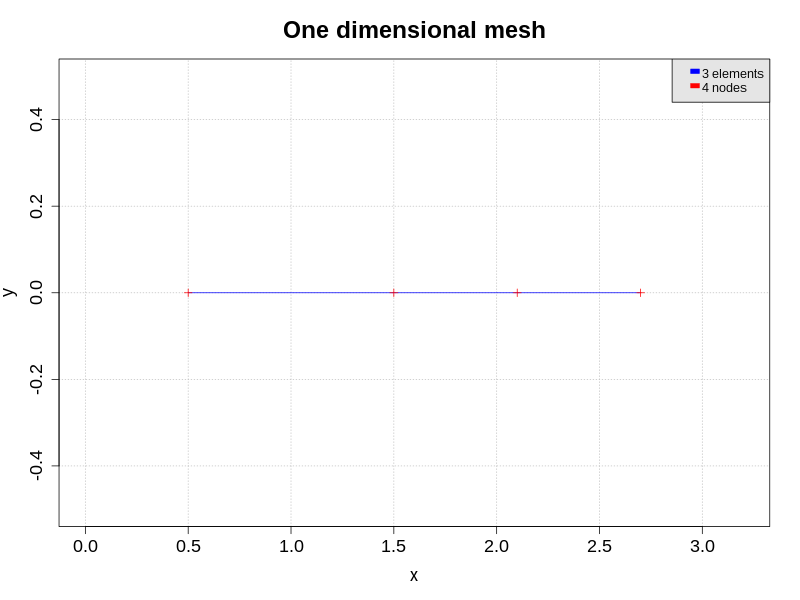
\includegraphics[width=7cm]{Figures/mesh_oneD.png}
      \caption{A mesh in dimension 1.}
      \label{mesh_oneD}
    \end{center}
  \end{minipage}
  \hfill
  \begin{minipage}{9cm}
    \begin{center}
      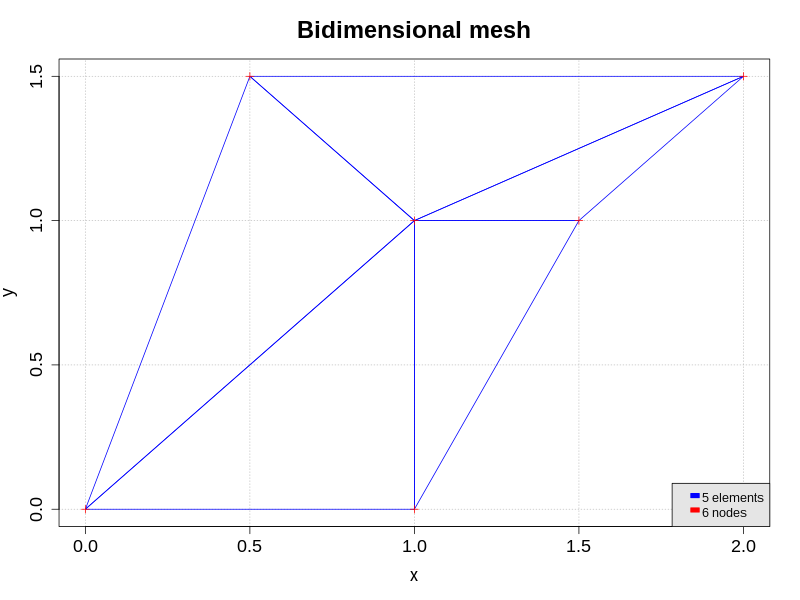
\includegraphics[width=7cm]{Figures/mesh_twoD.png}
      \caption{A mesh in dimension 2.}
      \label{mesh_twoD}
    \end{center}
  \end{minipage}
\end{figure}



\begin{figure}[H]
  \begin{minipage}{9cm}
  \begin{center}
    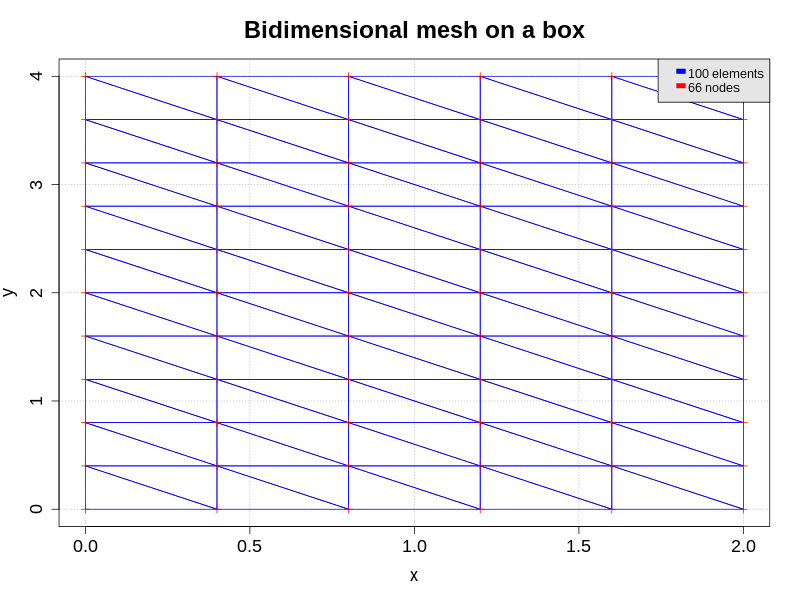
\includegraphics[width=7cm]{Figures/meshBox.png}
    \caption{A mesh defined from a Box.}
    \label{meshBox}
  \end{center}
  \end{minipage}
  \hfill
  \begin{minipage}{9cm}
  \begin{center}
    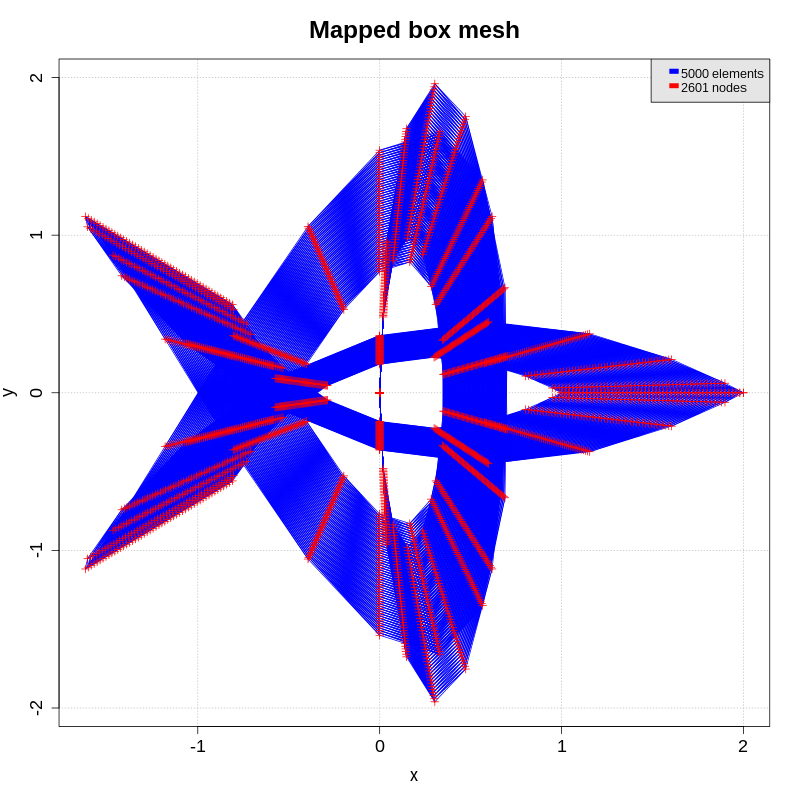
\includegraphics[width=7cm]{Figures/MappedBox.png}
    \caption{A box mesh mapped through  $f(r,  \theta)=(r\cos \theta \cos 5\theta, r\sin \theta \sin 5\theta)$.}
    \label{MappedBox}
  \end{center}
  \end{minipage}
\end{figure}

\begin{figure}[H]
  \begin{center}
    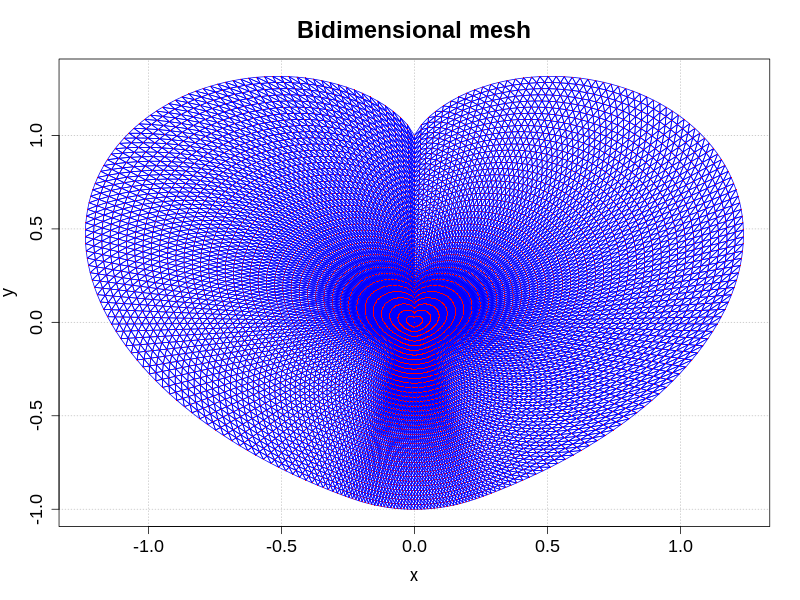
\includegraphics[width=7cm]{Figures/meshHeart.png}
    \caption{A mesh in dimension 2.}
    \label{meshHeart}
  \end{center}
\end{figure}